\section{Conditions de travail} \label{sec:conditions_travail}

\subsection{Présentation de l'équipe de développement} \label{sec:presentation_equipe}

Lors de mon stage de fin d'études, j'ai intégré une équipe de développement située dans un open space dans les bureaux
de l'agence Alltech Bordeaux, à Tourny. Nous étions en relation avec une autre équipe de développement à Cuba, ce qui
poussait la taille de l'équipe de MARS à varier de deux à trois. Sur place, à Bordeaux, nous étions deux, moi même et 
le chef de projet en charge de MARS, et nous avions parfois de l'aide de la part de développeurs cubains. 

\subsection{Organisation SCRUM} \label{sec:organisation_scrum}

Pour ce qui est de l'organisation sur le projet, nous utilisions le logiciel \texttt{Zoho} permettant une application
de la méthode SCRUM plus simple sur le projet. Toutes les semaines, nous avons effectué des \textit{réunions 
commerciales} où l'on présentait les changements apportés à MARS, ce qu'il reste a faire sur le sprint actuel et 
discuter avec les utilisateurs (clients) du logiciel sur les prochaines features à implémenter. Le rythme des réunions
étant de une par semaine, nous avons trouvé avantageux de fixer la durée des sprints de ce même temps. Pour ce qui est 
des tâches, elles étaient définies par le chef de projet, avec le quel je n'avais pas de soucis à communiquer en cas 
d'ambigüité\footnote{Même si celà était assez rare} ou si en cours d'implémentation, je trouvais pertinent de modifier
certains éléments de la tâche.

\subsection{Organisation des sources} \label{sec:organisation_sources}

Pour le code, nous utilisions git, sur un serveur local gitlab. Pour ce qui est de l'organisation des branches, nous 
utilisions le modèle \texttt{git flow}. Ce modèle repose sur le principe de construire une branche par tâche / feature 
puis de les merge sur une branche \texttt{develop} une fois terminées. Une fois à la fin d'un sprint, la branche 
develop est alors vérifiée puis merge sur une autre branche master pour ensuite être déployée (voir figure 
\ref{fig:gitflow}).

\begin{figure}[H]
    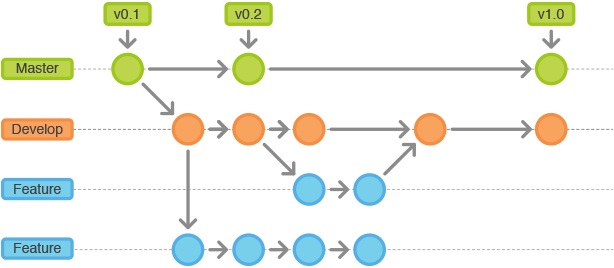
\includegraphics[width=\linewidth]{images/gitflow.png}
    \caption{Représentation du modèle Git Flow}\label{fig:gitflow}
\end{figure}